\section{Analysis Example}
\label{sec:example}

\begin{figure*}[htb]
\centering 
{\renewcommand\thelstnumber{%
\ifnum\value{lstnumber}>29\relax \the\numexpr  
278+\value{lstnumber}\relax\else 
\ifnum\value{lstnumber}>25\relax \the\numexpr  
139+\value{lstnumber}\relax\else 
\ifnum\value{lstnumber}>22\relax \the\numexpr  
132+\value{lstnumber}\relax\else 
\ifnum\value{lstnumber}>20\relax \the\numexpr  
130+\value{lstnumber}\relax\else 
\ifnum\value{lstnumber}>7\relax \the\numexpr  
92+\value{lstnumber}\relax\else 
\the\numexpr  
6+\value{lstnumber}\fi\fi\fi\fi\fi}
\lstinputlisting[language=Python,escapechar=|]{./example.py}}
\caption{Code example from GitHub}
\label{running_example}
\end{figure*}

Figure~\ref{running_example} from GitHub brings out some of the analysis  
challenges in constructing a knowledge graph for dynamic languages such as Python.  
The illustrative code shows a simple example in which a CSV file is  
first read using the Pandas library on line~\ref{line:read}, then some  
matrix computations are performed on the data using Numpy on  
line~\ref{line:mat}, and then it is passed to {\tt ann\_show} for  
visualization at line~\ref{line:plotcall}.  After adjusting based on  
the type of the data starting at line~\ref{line:lencall}, the computed data is  
displayed using Matplotlib on line~\ref{line:plot}.  These libraries  
are imported at lines~\ref{line:importplt},~\ref{line:importnp}, and~\ref{line:importpd}.  We want to  
capture this common usage pattern of {\tt plot} for instance in our knowledge  
graph. 

\begin{figure*}[htb]
\begin{center}
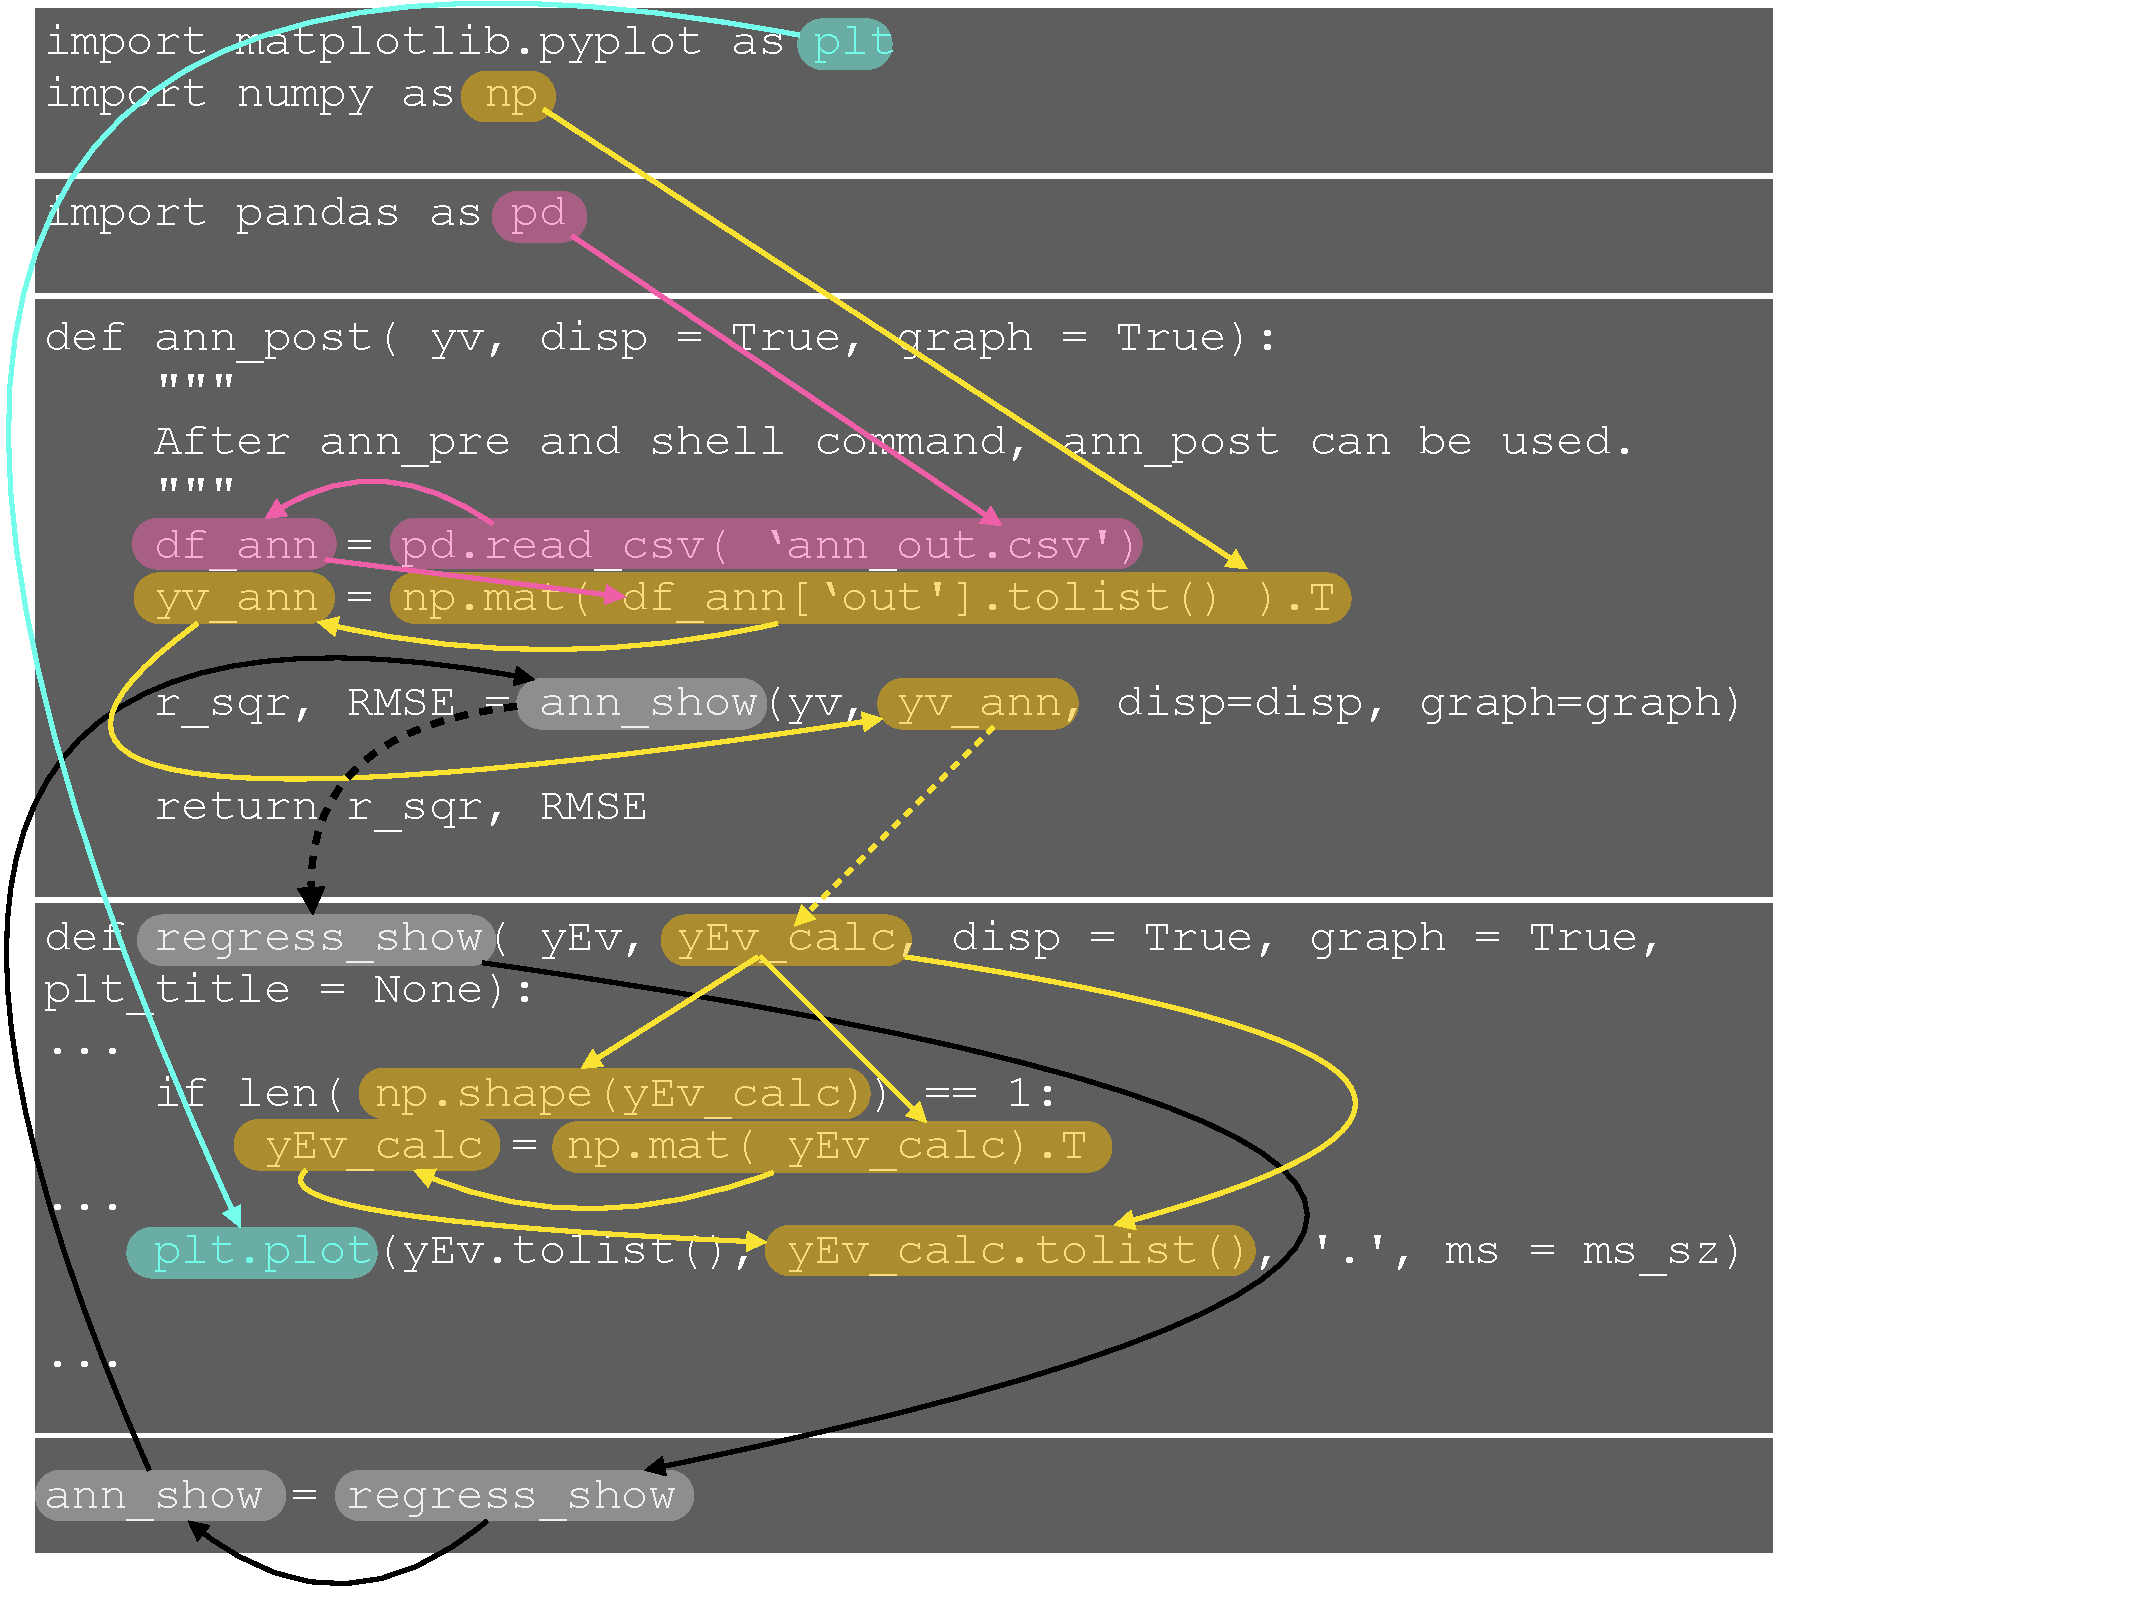
\includegraphics[width=5in]{paper_figures/example_flow}
\end{center}
\caption{Dataflow in example}
\label{fig:code_graph}
\end{figure*}

 The first thing to note is that the code in this snippet is in five
disparate pieces spread over roughly 200 lines of the source file.  Techniques
based on source text or local structures such as ASTs or CFGs will not
be able to capture dependencies over this range.  Global structures like a
call graph and dataflow analysis can.  Consider the call to {\tt ann\_show} on
line~\ref{line:ann_show}; it clearly calls the function {\tt
regress\_show} since that function is assigned to {\tt ann\_show}.
Knowing this requires following the dataflow from the definition of
{\tt regress\_show}, to its subsequent read, to the definition of {\tt
ann\_show}, to its read.  Thus dataflow must be tracked globally
across disparate portions of the code, as illustrated by the black
lines and boxes in Figure~\ref{fig:code_graph}.  And the call graph
must reflect that the function called depends on this dataflow, since
the call is to {\tt regress\_show} due to the dataflow, as illustrated
with the dashed arrow.  This is all complicated by the dynamic
nature of Python, illustrated here by the assignment of the function
{\tt regress\_show} to the variable {\tt ann\_show} on
line~\ref{line:ann_show}.  Note that {\tt ann\_show} called on
line~\ref{line:plotcall} is not even a function at all, but rather a variable
assigned from the actual function.  Of the analysis frameworks that
support interprocedural analysis including first class functions,
relatively few have been applied to Python.  We use WALA, which has, and supports many languages such as Javascript and Java.

This snippet also illustrates the fact that user code tends to rely heavily on imported library code, which is the main focus of what we represent in the knowledge graph.  There are seven lines of user code, and these lines
make use of three libraries ---{\tt Pandas}, {\tt Numpy}, {\tt
Matplotlib}---and four functions from them---{\tt read\_csv}, {\tt
mat}, {\tt to\_list}, {\tt plot}---with {\tt to\_list} being used
three times.  The interplay of dataflow between the user code and its
library calls is intricate and crucial to understanding dataflow.
Consider what is required even to know that {\tt pyplot} is used on an
object from {\tt numpy}.  The first step is straightforward dataflow
from the {\tt import} call to {\tt np.mat}, shown by a yellow arrow.
The {\tt mat} returns some object created by {\tt numpy} and then its
{\tt T} field is extracted and assigned to {\tt yv\_ann}.  So {\tt
yv\_ann} is created by {\tt numpy}, show by a yellow arrow to it.
That same value is used in the {\tt ann\_show} call, with another
yellow arrow connecting it.  We saw above how the call target was
determined, so a dashed yellow arrow connects argument {\tt yv\_ann}
to parameter {\tt yEv\_calc}.  The dataflow in {\tt regress\_show} is
similar, with dataflow via {\tt yEv\_calc} and another value from {\tt
numpy} created by {\tt np.mat}.  The last step is the dataflow from
the {\tt pyplot} import to the {\tt plt.plot} call, where it is clear
that a call to {\tt pyplot} is using a value from {\tt numpy}.

The foregoing seems to assume we understand dataflow through the library
calls, but any actual model of code within the libraries will be daunting.  Any
actual analysis of the code must contend with a large code base in
multiple languages that are used to implement libraries.  
And any model will be difficult due to the sheer
scope of the libraries, with thousands of calls in each library alone.  There
is no formal static typing in this code to help; there is
idiosyncratic English API documentation of varying quality, but the
precise parametric semantics of functions like {\tt to\_list} is hard
to capture robustly in human- and machine-comprehensible English.  And
yet we need to capture enough library semantics to understand dataflow
at a high level.

To just approximate dataflow, we use an approach where 
the precise meanings of library calls do
not always matter as long as we track the flow of objects between
different calls.  For instance, since we want to capture that {\tt
plot} is used on the result of a {\tt mat} call, we need to track
data flow.  We really want an object that represents whatever it may
be that {\tt mat} returns.  Beyond that, we need to follow accesses to
that object, such as the read of {\tt T} on line~\ref{line:mat}.  To
do this, we introduce turtle objects: every library call returns a fresh
turtle, and accesses to properties---such as {\tt T}--- return the
same unknown object as its container.  Thus the calls on {\tt
  read\_csv}, {\tt mat}, {\tt to\_list}, and {\tt plot} all return new
turtle objects.  On the other hand, user code objects, such as the
function {\tt regress\_show} are treated normally.  As we show, this
mechanism allows us to track data flow with sufficient precision
without needing to model APIs at all.  Approximate analysis is what we use to scale analysis to many thousands of library calls in building our knowledge graph.
